%&format -translate-file pdf
\documentclass{article}
\usepackage{graphicx}
\usepackage{listings}
\lstset{basicstyle=\ttfamily\tiny}
\title{Project 2}
\author{RT Hatfield}
\date{29 September 2016}
\begin{document}
\maketitle
\begin{itemize}
    \item My code doesn't quite work.  There's some deep-seated bug I couldn't fix.  I think it has to do with 
    the ordering of points in a hull.
    \begin{lstlisting}
using System;
using System.Drawing;
using System.Collections.Generic;
using System.Linq;
using System.Text;
using System.Windows.Forms;

namespace _1_convex_hull
{
    class CHull
    {
        List<PointF> points;
        int indexOfCurrentPoint = -1;
        // we always start with the leftmost point at 0, we set rightmost later
        int indexOfLeftmostPoint = 0;
        int indexOfRightmostPoint = -1;

        int topRight = -1;
        int topLeft = -1;
        int bottomRight = -1;
        int bottomLeft = -1;

        public CHull(List<PointF> pointList)
        {
            // points should already be sorted by X value
            PointF right = pointList.Last();
            PointF left = pointList.First();
            // temporarily remove the left point to not calculate slope of itself, divide-by-zero
            pointList.Remove(left);
            points = pointList.OrderByDescending(x => calculateSlope(left, x)).ToList(); // O(nlogn) again, must be, right?
            points.Insert(0, left);

            this.indexOfRightmostPoint = points.IndexOf(right);
        }

        public CHull merge(CHull other)
        {
 
            // find all four "bridge" points
            // starting with the upper right, go clockwise and just make a new list

            // Find upper bridge:
            //  Start with rightmost point on this hull and leftmost point on other hull
            //  This runs up to n times, so O(n).  The inner part can be up to O(n), also.
            //  Worst case: O(n^2)
            this.indexOfCurrentPoint = this.indexOfRightmostPoint;
            other.indexOfCurrentPoint = other.indexOfLeftmostPoint;
            bool rightHasChanged = true;
            bool leftHasChanged = true;
            
            while (rightHasChanged || leftHasChanged) 
            {
                bool unchanged = false;

                if (leftHasChanged)
                {
                    leftHasChanged = false;
                    topRight = findtopRight(other);
                    if (other.points[topRight].Equals(other.points[other.indexOfCurrentPoint]))
                    {
                        // wait, we didn't actually update anything, so...
                        unchanged = true;
                    }
                    else
                    {
                        rightHasChanged = true;
                        other.indexOfCurrentPoint = topRight;
                    }
                }
                if (rightHasChanged)
                {
                    rightHasChanged = false;
                    topLeft = findtopLeft(other);
                    if (points[topLeft].Equals(points[this.indexOfCurrentPoint]))
                    {
                        // we didn't actually find a new point.  won't repeat.
                        unchanged = true;
                    }
                    else
                    {
                        leftHasChanged = true;
                        this.indexOfCurrentPoint = topLeft;
                    }
                }

                if (unchanged)
                {
                    leftHasChanged = false;
                    rightHasChanged = false;
                }
            }

            // Now find lower bridge.  Same complexity as earlier
            this.indexOfCurrentPoint = this.indexOfRightmostPoint;
            other.indexOfCurrentPoint = other.indexOfLeftmostPoint;
            rightHasChanged = true;
            leftHasChanged = true;
            
            while (rightHasChanged || leftHasChanged)
            {
                bool unchanged = false;

                if (leftHasChanged)
                {
                    leftHasChanged = false;
                    bottomRight = findbottomRight(other);
                    if (other.points[bottomRight].Equals(other.points[other.indexOfCurrentPoint]))
                    {
                        // haven't found a new point
                        unchanged = true;
                    }
                    else
                    {
                        rightHasChanged = true;
                        other.indexOfCurrentPoint = bottomRight;
                    }
                }

                if (rightHasChanged)
                {
                    rightHasChanged = false;
                    bottomLeft = findbottomLeft(other);
                    if (this.points[bottomLeft].Equals(this.points[this.indexOfCurrentPoint]))
                    {
                        unchanged = true;
                    }
                    else
                    {
                        leftHasChanged = true;
                        this.indexOfCurrentPoint = bottomLeft;
                    }
                }

                if (unchanged)
                {
                    leftHasChanged = false;
                    rightHasChanged = false;
                }
            }

            // reconstruct the hull: go around from the leftmost, add the top bridge, 
            //      go around the right hull, add the lower bridge, and continue until
            //      there's a cycle.
            // this part should run in O(n) time
            List<PointF> combined = new List<PointF>();
            for (int i = 0; i <= topLeft; i++)
            {
                combined.Add(this.points[i]);
            }
            for (int i = topRight; i < other.points.Count; i++)
            {
                i = Math.Abs(i % other.points.Count);
                combined.Add(other.points[i]);
            }
            combined.Add(other.points[bottomRight]);
            for (int i = bottomLeft; i != 1; i++)
            {
                i = i % this.points.Count;
                combined.Add(this.points[i]);
            }

            return new CHull(combined);
        }

        public void drawHull()
        {
            if (points != null && points.Count > 0)
            {
                List<PointF> tempPoints = new List<PointF>(points);
                tempPoints.Add(points.First());
                _2_convex_hull.ConvexHullSolver.getGraphics().DrawLines(new Pen(Brushes.LimeGreen), tempPoints.ToArray());
            }
        }

        private int findtopRight(CHull other) // this method (and all the others like it) run in O(n) time.
        {
            // using pivot as anchor (left end, should be leftmost point of this)
            //      we drage the free end around the other hull until we get maximum slope
            int anchor = this.indexOfCurrentPoint;
            int free = other.indexOfCurrentPoint;

            // we can't simply increment, because it's a "clock"
            int mod = other.points.Count;

            while (calculateSlope(this.points[anchor], other.points[(free + 1) % mod]) > 
                    calculateSlope(this.points[anchor], other.points[free]))
            {
                free = (free + 1) % mod;
            }

            return free;
        }

        private int findbottomRight(CHull other)
        {
            int anchor = this.indexOfCurrentPoint;
            int free = other.indexOfCurrentPoint;

            int mod = other.points.Count;

            while (calculateSlope(this.points[anchor], other.points[Math.Abs((free - 1) % mod)]) <
                    calculateSlope(this.points[anchor], other.points[free]))
            {
                free = Math.Abs((free - 1) % mod);
            }

            return free;
        }

        private int findtopLeft(CHull other)
        {
            int anchor = other.indexOfCurrentPoint;
            int free = this.indexOfCurrentPoint;

            int mod = this.points.Count;

            while (calculateSlope(this.points[Math.Abs((free + 1) % mod)], other.points[anchor]) <
                    calculateSlope(this.points[free], other.points[anchor]))
            {
                free = Math.Abs((free + 1) % mod);
            }

            return free;
        }

        private int findbottomLeft(CHull other)
        {
            int anchor = other.indexOfCurrentPoint;
            int free = this.indexOfCurrentPoint;

            int mod = this.points.Count;

            while (calculateSlope( this.points[Math.Abs((free + 1) % mod)], other.points[anchor]) >
                    calculateSlope(this.points[free], other.points[anchor]))
            {
                free = Math.Abs((free + 1) % mod);
            }

            return free;
        }

        public static float calculateSlope(PointF left, PointF right) // constant time
        {
            return -(right.Y - left.Y) / (right.X - left.X);
        }
    }
}

using System;
using System.Collections.Generic;
using System.Text;
using System.Linq;
using System.Drawing;
using _1_convex_hull;

namespace _2_convex_hull
{
    class ConvexHullSolver
    {
        static System.Drawing.Graphics _g;
        System.Windows.Forms.PictureBox pictureBoxView;
        public static ConvexHullSolver _instance;

        public ConvexHullSolver(System.Drawing.Graphics g, System.Windows.Forms.PictureBox pictureBoxView)
        {
            _instance = this; // make a sort of singleton so we can draw right from the CHull
            _g = g;
            this.pictureBoxView = pictureBoxView;
        }

        public static System.Drawing.Graphics getGraphics()
        {
            return _g;
        }

        public void Refresh()
        {
            // Use this especially for debugging and whenever you want to see what you have drawn so far
            pictureBoxView.Refresh();
        }

        public void Pause(int milliseconds)
        {
            // Use this especially for debugging and to animate your algorithm slowly
            pictureBoxView.Refresh();
            System.Threading.Thread.Sleep(milliseconds);
        }

        public void Solve(List<System.Drawing.PointF> pointList)
        {
            List<PointF> sortedPoints = pointList.OrderBy(p => p.X).ToList();
                // the complexity of OrderBy isn't given in documentation, but 
                //  I assume Microsoft isn't putting crap code in C#, so it must be no 
                //  worse than O(nlogn)
            CHull convexHull = getHull(sortedPoints);
            convexHull.drawHull();
        }

        private CHull getHull(List<System.Drawing.PointF> pointList)
        {
            // recursive method: split the hull in half, call getHull on each half, merge.
            // base case: 2 or 3 points.  just return a new CHull
            // otherwise: split list into L and R
            //              call getHull on each list to get LHull and RHull
            //              call LHull.merge(RHull);
            
            if (pointList.Count < 4)
            {
                // base case
                return new CHull(pointList);
            }

            else
            {
                // we don't need to worry about the EXACT midpoint (no special handling of odd-length list)
                // because call tree doesn't need to be balanced
                List<PointF> LPoints = new List<PointF>(pointList.Take<PointF>(pointList.Count / 2));
                List<PointF> RPoints = new List<PointF>(pointList.Skip<PointF>(pointList.Count / 2));

                CHull LHull = getHull(LPoints);
                CHull RHull = getHull(RPoints);

                return LHull.merge(RHull);

                /*
                 * This algorithm gets two subproblems of 1/2 size, and then joins them in (worst-case) quadratic time.
                 */
            }
        }
    }
}
    \end{lstlisting}
    \item I see that I have 2 subproblems of $\frac{1}{2}$ size, which I'm joining in quadratic time.  Therefore,
    I have complexity: $$2T(\lceil\frac{n}{2}\rceil) + O(n^2)$$ $$2 > log_2^2$$ $$T(n) = O(n^2)$$
    \item Since my code didn't work properly, I did not gather experimental data.  
    \item See Figure 1 and Figure 2.
    \begin{figure}[p]
        \centering
        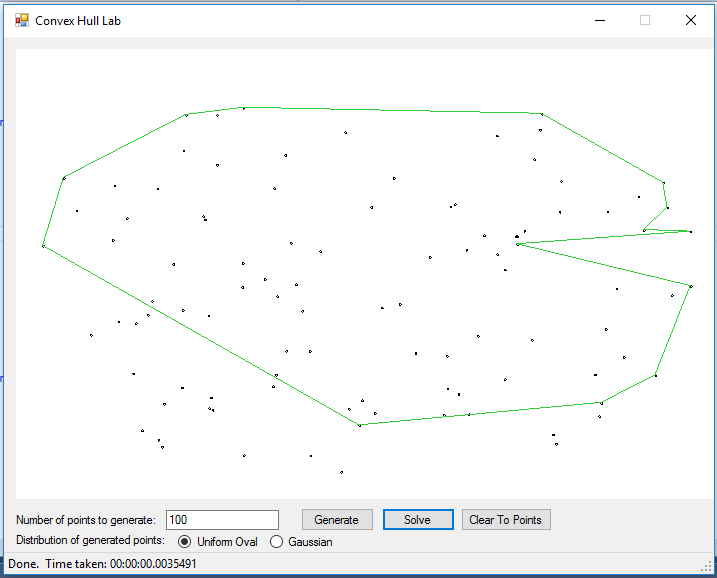
\includegraphics[resolution=72, width=\textwidth]{100}
        \caption{100 points}
    \end{figure}
        \begin{figure}[p]
        \centering
        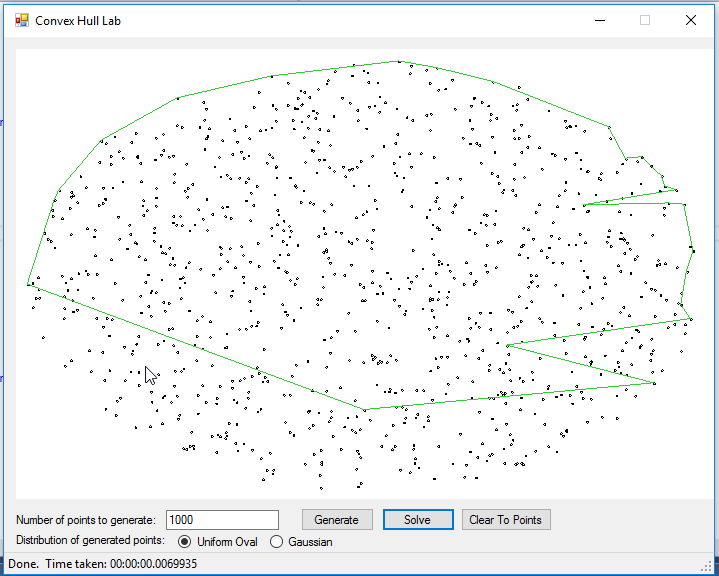
\includegraphics[resolution=72, width=\textwidth]{1000}
        \caption{1000 points}
    \end{figure}
\end{itemize}
\end{document}
